\section{方位角取得の実験}
\label{chap:exp_azimuth_angle}
\subsection{実験のセッティング}
\label{sec:anechoic_chamber}
\subsubsection{実験の目的}\label{exp_popse}
今回の実験の評価項目としては以下の3点について実験をそれぞれ行い、評価を行う。
\begin{description}
  \item[(1)] 実環境下(無響室)での中域、高域のエネルギーの大きさの変化の計測値とモデルの差
  \item[(2)] 実環境下での中域、高域のエネルギー比と方位角の関係性の計測値からの計算結果とモデルの差
  \item[(3)] 方位角の推定結果と実際の方位角の差
\end{description}

\subsubsection{実験環境}
本実験は無響室と実際の屋内の部屋の二通りで実験を行った.\\
無響室は、大阪産業技術研究所和泉センター[ ?? ]の無響室を使用した。実験環境の図を\figref{chamber}に示す。\\
また、屋内の部屋として、奈良先端科学技術大学院大学情報科学棟S1教室を使用した。このとき、机や椅子といったものはすべて除外している。このときの環境の様子の図を\figref{room}に示す。\\

\begin{figure}[tb]
    \centering
    \subfigure[Anechoic chamber]{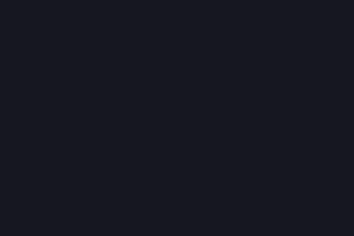
\includegraphics[width=55mm]{images/fig_sample.png}}
    \label{fig:chamber}
    \subfigure[NAIST S1 room]{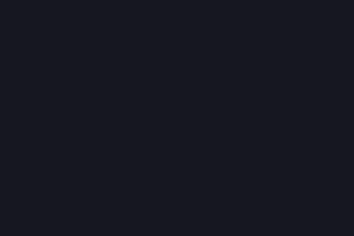
\includegraphics[width=55mm]{images/fig_sample.png}}
    \label{fig:room}
    \caption{Experiment Images}
    \label{fig:exp_photo}
\end{figure}

実験に用いた道具は以下の通りである。
\begin{itemize}
	\item マイク:Seed社製 Respearker Mic Array V2.0
	\item スピーカ:FPS社製 コンパクトオーディオスピーカー(SW5500-SS)
    \item 回転台:シグマ光機社製 小型回転ステージ(OSMS-60YAW)
    \item 平面:ガラス板(横40×縦25)
\end{itemize}
マイクは4つのマイクロホンを搭載しあたマイクロホンアレイを用いた。理由としては、Beamforming技術を用いることで音源の到来方向を制限するためである。今回、スピーカをマイクと対象平面とは180[deg]反対側に配置した。これにより、Beamformingを用いることで、スピーカ側180[deg]の音源を取らないように制限することができる。これにより、直接音を弱め、反射音を強めることができると考えた。

スピーカは平面波スピーカを使用している。普段、音は近傍界、遠方界によって波の形状が変化する。近傍界では球面波、遠方界では平面波となる。今回の手法を用いる場合、音源の入射方向が一意に決まる必要があるため、平面波を用いることが必要である。そのため、平面波を出力の時点で出すことができるスピーカを用いることでこの問題を解決した

回転台は\ref{exp_popse}節の(1),(2)において平面の方位角との収録音の関係を取得する際に方位角に関して、1[deg]ごとに変化させた実験データ収録するために使用した。今回使用した回転台は最小単位が0.0001[deg]の精度で回転させることができる。そのため、今回欲しい平面の方位角を1[deg]ごとに-50[deg] $\sim$ 50[deg]を取るには十分だと考えている。また、停止時の振動と移動時の雑音も少ないため、今回のような音を使った実験を行うのに最適だと考えた。
さらに、本実験ではバックラッシュ誤差が少しでも出ないように1[deg]を連続で変化させるのではなく、10[deg]ずつ変化させ、データを集めた。

平面にはガラス板を用いた。理由としては、ガラスは音の反射率も高いからである。更に、ガラスはカメラでの認識が難しいため、音を使う優位性があると考えた。
その他の実験をした際のパラメータを表\ref{tab:para}に示す

\begin{table}[t]
    \centering
    \caption{Parametar of experiment}
    \begin{tabular}{|c|c|}\hline
        $_\phi[\mathrm{deg}]$ & 90 \\ \hline
        $\psi[\mathrm{deg}]$ & $-50 \sim 50$ \\\hline
        % $\rho$ & 0.9 \\\hline
    \end{tabular}
    \label{tab:para}
\end{table}

実験の様子を図\ref{fig:exp_env}に示す。

\begin{figure}[t]
  \begin{center}
  \vspace{1zh}
    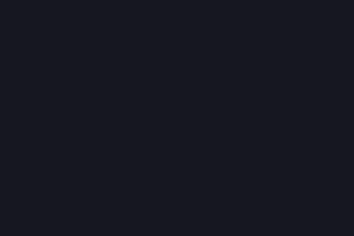
\includegraphics[width=0.7\linewidth]{images/fig_sample.png}   
  \end{center}
  \caption{Experiment environment}
  \label{fig:exp_env}
\end{figure}

\subsubsection{実験方法}
二通りの実験を行った。
まず、(1)に関してはスピーカからTSP信号をもちいた伝達関数の作成を行った。
本実験では、TSP信号を用いてインパルス応答を求めることで伝達関数を作成する。この伝達関数とモデルとを比較することによってモデルを評価する。また、今回はインパルス応答の周波数特性を見たいため、Up-TSP信号を用いた。

次に(2)、(3)に関しては、スピーカから1000[Hz], 2000[Hz], 5000[Hz]をならすことで、方位角を推定した。
本実験では、方位角を求めるために必要な中域($f_m$ = 1000)、高域($f_h$ = 2000, 5000)の周波数をそれぞれ0.05[s]ずつならした音の反射音を取得することで、方位角$N$を求めて、モデルを評価する。
今回時間を0.05[s]にした理由としては、反射音と直接音の干渉を少なくすることを目的としている。今回、マイク、反射面間の距離は20[cm]にしているため完全に干渉をなくすためには44100[Hz]でスピーカから音を出力する必要があった。しかし、スピーカの性能面から16000[Hz]が限界であったことと1000[Hz]という音を出力する際にあまりに短いと音が潰れてしまうことの2点があった。そのため、今回は余裕を持って0.05[s]のパルス波を使用した。

\subsection{モデルを用いた場合の評価}
\label{sec:result_model}
\subsubsection{中、高域のエネルギーの変化}
(1)について、図\ref{fig:result1}はTSP信号を用いて作成したインパルス応答です。計算方法は時間領域をそのままフーリエ変換した(周波数幅44100)。その後、フーリエ変換の結果を$-50 \leq \psi <50$の100データの各周波数成分の平均を取り、その平均で割った結果の中でも$\psi=0, \psi=20$の値を描画したものです。
結果より、直接音の影響が大きい点と今回行った処理が根拠に基づいていない点の2点より図\ref{fig:e-f}のような結果は出なかったと考えられる。また、今回の処理では、同様に方位角への変化も見ることはできなかった。

\begin{figure}[t]
  \begin{center}
  \vspace{1zh}
    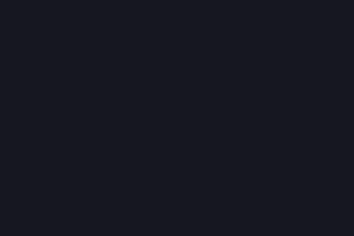
\includegraphics[width=0.7\linewidth]{images/fig_sample.png}   
  \end{center}
  \caption{elationship between energy (E) change with respect to frequency (f) and azimuth direction (N) when the sound source direction (S) and microphone direction (V)}
  \label{fig:result1}
\end{figure}

\subsubsection{エネルギー比と方位角の関係}
(2)について、図\ref{fig:result2}に示す。バンドパスフィルタをかけた結果のRMSの値を1000, 2000で割った値である。しかし、以上に0付近で大きくなっている。これは計算結果の誤りであると考えられる。

\begin{figure}[t]
  \begin{center}
  \vspace{1zh}
    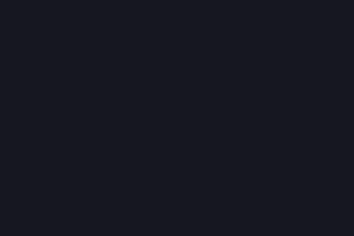
\includegraphics[width=0.7\linewidth]{images/fig_sample.png}   
  \end{center}
  \caption{Relation between energy ratio $D(\mathbf{N}|f_m, f_h)$ and azimuth angle $\mathbf{N}$ between mid and high frequencies at a point Q on the plane($f_m = 1000$, $f_h = 2000$)}
  \label{fig:result2}
\end{figure}

\subsubsection{方位角の推定}
(3)について、(1),(2)の結果が上手く出ていないため、導出することができていない。

% \begin{figure}[t]  
%   \begin{center}
%   \vspace{1zh}
%     \includegraphics[width=\linewidth]{fig.eps}   
%   \end{center}
%   \caption{Experiment environment}
%   \label{fig:result3}
% \end{figure}

\subsection{モデル作成に関する考察}
 理論通りの結果にならない原因としては直接音の影響が大きいことがあると考える。現状完全に反射音のみを取得しているのではなく、マイクには直接音と反射音の合成音が取得されている。この直接音と合成音の分離が必要だと考える。この分離する手法としては2つ考えられる。1点目はスピーカからの距離と物体までの距離がわかっている場合、直接音のみのデータを録音しておく。スピーカとマイクの出力に関して同期を取ることで音速よりマイクへの音の到達時間を計算し、音データの中でも直接音が取得される時点から直接音のみのデータを引く。2点目はBeamformerを用いた音域制限である。現在使用しているデータはマイクで取得されたデータをそのまま用いている。理論的には、ある一点Qからの音のみを知りたいため、Beamformingを用いることによって取得する方向を制限することができ、これにより直接音の影響を完全に消す事はできないが弱めることができると考えられる。

\subsection{SVRを用いての評価}
\label{sec:result_svr}
SVRを用いての結果を\figref{result_svr_1}に示す。このとき、横軸は実際の対象面の角度、縦軸は推定した対象面の角度である。つまり、正解の値はオレンジの線のような直線がかけることがわかる。そのため、求める結果としては、このオレンジの線にどれだけ沿っているのかを評価する。

\begin{figure}[tb]
    \centering
    \subfigure[Result using SVR anechoic data]{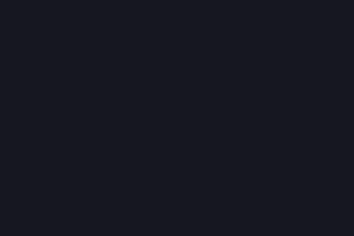
\includegraphics[width=0.7\linewidth]{images/fig_sample.png}}
    \label{fig:result_svr_anechoic}
    \vspace{2zh}
    \subfigure[Result using SVR real
    data]{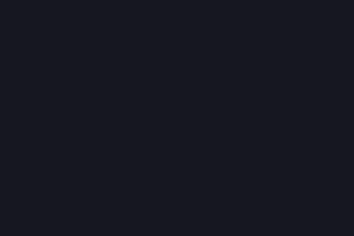
\includegraphics[width=0.7\linewidth]{images/fig_sample.png}}
    \label{fig:result_svr_real}
    \vspace{1zh}
    \caption{Result of Experiment based on SVR}
    \label{fig:result_svr_1}
\end{figure}

次に、無響室で作成したモデルを実環境での実験データでも予測ができるのかを検証した。その結果を\figref{result_svr_2}に示す。

このときのそれぞれの決定係数(Coefficient of determination, $\mathrm{R}^2$)と二乗平均平方誤差(Root Meen Squared Error, RMSE [deg])で評価した結果をTable. \ref{tab:result_svr_r2_rmse}に示す。

\begin{table}[tb]
\caption{Result of SVR}    
\vspace{1zh}
\centering
  \begin{tabular}{|l|p{6em}|p{6em}|} \hline
    Traing data/ Test data & $\mathrm{R}^2$ & RMSE [deg] \\ \hline\hline 
    Anechoic / Anechoic & 0.8 &  3.5 \\ \hline 
    Real / Real & 0.7 &  4.0 \\ \hline
    Anechoic / Real & 0.7 &  4.5 \\ \hline
  \end{tabular}
  \label{tab:result_svr_r2_rmse}
\end{table}

\clearpage

\begin{figure}[tb]
  \begin{center}
  \vspace{1zh}
    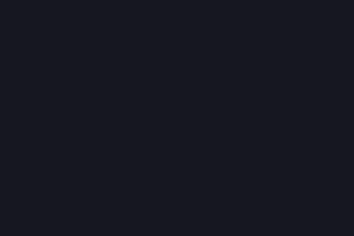
\includegraphics[width=0.7\linewidth]{images/fig_sample.png}   
  \end{center}
  \caption{Result using SVR (traing data: anechoic data, test data: real data)}
  \label{fig:result_svr_2}
\end{figure}


このように、SVRを用いることによって、5 [deg]以下の誤差で推定することができることがわかった。しかし、現状の実験で用いているものが最適であるかはわからない。そこで、実験設定について、正しかったのかの検証を行う。\\
使用した音の種類、周波数の範囲、スピーカについて、この組み合わせが正しかったのかを考察すべく、\secref{result_svr_sound_kind} $\sim$ \secref{result_svr_speaker}でそれぞれについて評価していく。

\subsubsection{使う音の評価}
\label{sec:result_svr_sound_kind}
今回、音波として、TSP信号を用いている。このような、周波数成分を多く持ったデータを使うことが有効であるかどうかを確認する。

方法は、単一の高さの音を流した音の場合でも同様にデータを作成し、SVRをつかってモデル化したモデルを用いて、推定を行い、その二乗平均平方誤差を比較する。
この結果を\figref{result_sound_kind}に示す。

\begin{figure}[tb]
    \centering
    \subfigure[1000Hz]{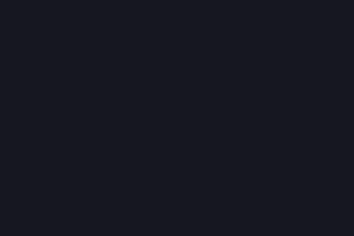
\includegraphics[width=55mm]{images/fig_sample.png}}
    \label{fig:1000[Hz]}
    \subfigure[2000Hz]{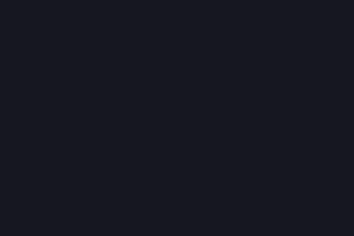
\includegraphics[width=55mm]{images/fig_sample.png}}
    \label{fig:2000[Hz]}
    \caption{Comparison of result about sound kinds}
    \label{fig:result_sound_kind}
\end{figure}

\subsubsection{使う周波数の範囲の評価}
\label{sec:result_svr_freq_renge}
今回、使用する音の周波数として、音の反射の特性の変化を用いるために1000 [Hz]から2000[Hz]の音波を使用した。今回、このような音を用いることが有効であるかどうかを確認する。

方法としては、二通りで検証する。\\
1つ目は1000[Hz]から8000[Hz]までの音を用いて、主成分分析を行い、それぞれの主成分における各変数の固有値の絶対値を比べる。\\
2つ目は1000[Hz]から1000[Hz]おきにこれまでと同様の方式でデータセットを作成し、それぞれの決定係数、二乗平均平方誤差を比較する。結果をそれぞれ\figref{result_freq_range_1}, \figref{result_freq_renge_2}に示す。

\begin{figure}[tb]
  \begin{center}
  \vspace{1zh}
    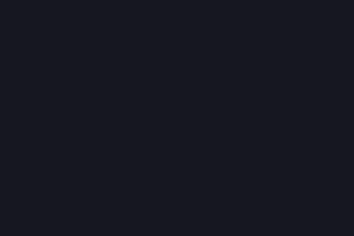
\includegraphics[width=0.4\linewidth]{images/fig_sample.png}   
  \end{center}
  \caption{Comparison of frequency range based on case PCA}
  \label{fig:result_freq_range_1}
\end{figure}

\begin{figure}[t]
    \subfigure[$1000$-$2000$Hz]{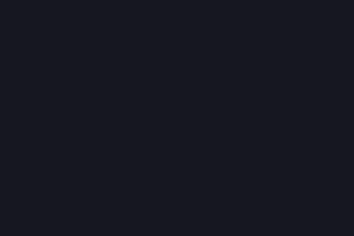
\includegraphics[width=0.35\linewidth]{images/fig_sample.png}
     \label{fig:1000}}
    \subfigure[$2000$-$3000$Hz]{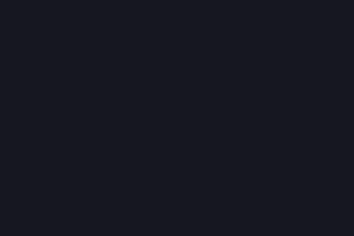
\includegraphics[width=0.35\linewidth]{images/fig_sample.png}
     \label{fig:2000}} 
    \subfigure[$3000$-$4000$Hz]{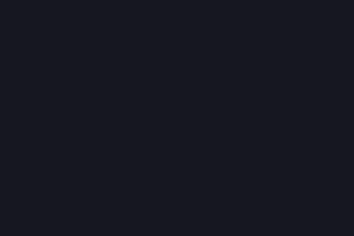
\includegraphics[width=0.35\linewidth]{images/fig_sample.png}
     \label{fig:3000}}
    \subfigure[$4000$-$5000$Hz]{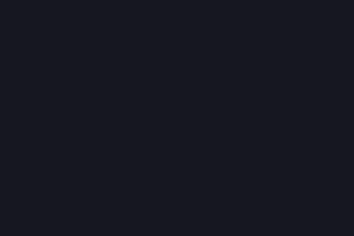
\includegraphics[width=0.35\linewidth]{images/fig_sample.png}
     \label{fig:4000}} 
    \subfigure[$5000$-$6000$Hz]{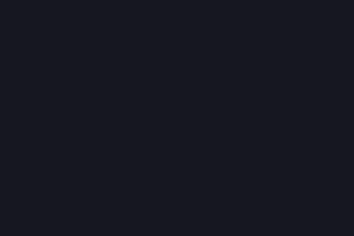
\includegraphics[width=0.35\linewidth]{images/fig_sample.png}
     \label{fig:5000}}  
     \subfigure[$6000$-$7000$Hz]{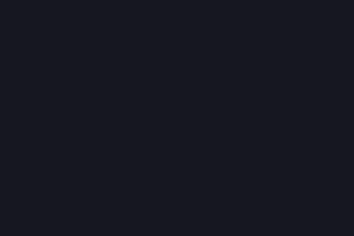
\includegraphics[width=0.35\linewidth]{images/fig_sample.png}
     \label{fig:6000}}     \subfigure[$7000$-$8000$Hz]{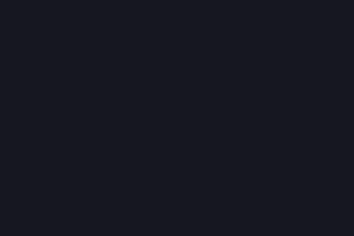
\includegraphics[width=0.35\linewidth]{images/fig_sample.png}
     \label{fig:7000}}    
     \caption{Comparison of frequency range based on case that I create models individually}
    \label{fig:result_freq_renge_2}
\end{figure}
\clearpage

\subsubsection{使うスピーカの評価}
\label{sec:result_svr_speaker}
今回の実験では、平面波のスピーカを用いている。しかし、これが球面波スピーカの場合ではどうなるのかを確認する。

方法は球面波スピーカで発した音のデータを同様に作成したものでSVRをもちいてモデルを作成した。このときのスピーカは??を用いている。??について、の図を用いた場合の実験環境を\figref{exp_spherical_wave}に示す。
この実験における結果を\figref{result_speaker_kinds}に示す

\begin{figure}[tb]
    \centering
    \subfigure[Speaker]{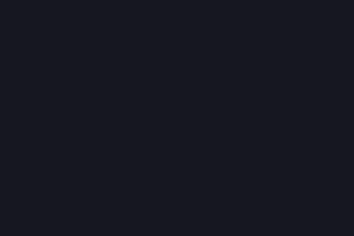
\includegraphics[width=55mm]{images/fig_sample.png}}
    \label{fig:spherical_speaker}
    \subfigure[Experiment environment]{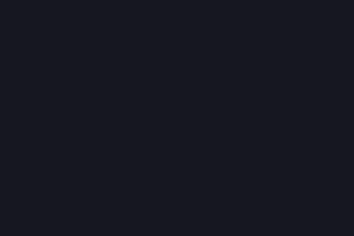
\includegraphics[width=55mm]{images/fig_sample.png}}
    \label{fig:exp_environment_spherical}
    \caption{Experiment for spherical wave}
    \label{fig:exp_spherical_wave}
\end{figure}

\begin{figure}[tb]
  \begin{center}
  \vspace{1zh}
    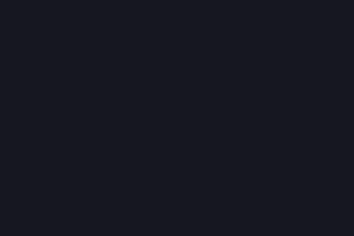
\includegraphics[width=0.6\linewidth]{images/fig_sample.png}   
  \end{center}
  \caption{Comparison of speaker kinds}
  \label{fig:result_speaker_kinds}
\end{figure}

\subsection{SVRを用いた場合の考察}
SVRを用いた場合、物体平面の面の方向を誤差5 [deg]以下で推定することができた。このように推定できた理由としては、物体平面の方位角と周波数領域の波の様子には連続的な関係があった。この連続的な関係については、\figref{relation_intensity_azimuth}に示す。
このような変化が1000 [Hz]から2000 [Hz]の間で見られた。そのため、このような変化の特徴を使うことでSVRでは推定モデルを作成することができたと考えている。

\begin{figure}[tb]
  \begin{center}
  \vspace{1zh}
    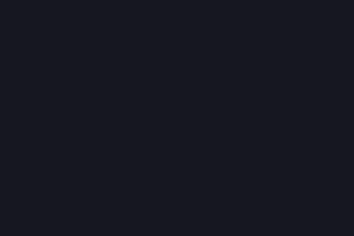
\includegraphics[width=0.5\linewidth]{images/fig_sample.png}   
  \end{center}
  \caption{Relationship of intensity and azimuth angle in 1000 [Hz]}
  \label{fig:relation_intensity_azimuth}
\end{figure}

しかし、このような変化はモデルを作成する際に考えていた変化とは違う。この理由として1点考えた。それは、モデル作成時はある1点における反射を元に考え、モデルを作成した。しかし、今回の取得した音は面から反射した音そのもので音を分離したものではない。そのため、Delay-Sum Beamforming を用いて、対象物体の中心から反射してきた音を分離してみた。その音を使い、方位角と波の強さの関係とSVRのモデルを作成し、推定した結果を\figref{beam_check}を示す。

\begin{figure}[tb]
    \centering
    \subfigure[Relationship of intensity and azimuth angle in 1000 Hz]{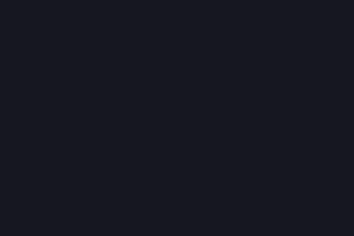
\includegraphics[width=55mm]{images/fig_sample.png}}
    \label{fig:beam_check_intensity}
    \subfigure[Experiment environment]{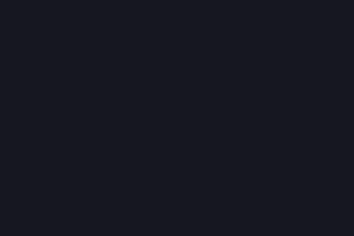
\includegraphics[width=55mm]{images/fig_sample.png}}
    \label{fig:beam_check_svr}
    \caption{Experiment for spherical wave}
    \label{fig:beam_check}
\end{figure}

この結果より、精度はBeamforming前よりも低下した。この理由としては、2点あると考えている。1点目はBeamforingの精度が悪い。[参考文献]より、4個のマイクアレイではほとんど分離が不可能であることがわかる。このように、分離の精度が悪いと考えられる。
2点目は、物体形状の影響が大きいという点である。物体形状の情報をわざと消しているBeamformingを用いることでその情報が落ち、精度が落ちたと考えられる。

このような結果より、3点の疑問点もできた。
\begin{itemize}
    \item 材質による影響はどの程度あるのか?
    \item 物体の大きさを小さくしても認識可能か?
    \item 複数面でも認識可能か?
\end{itemize}
上記の3点について、次の章で検証していく。

また、SVRにおいて、どの周波数に関係があるのか?、どのような関係が見えるかを調べるために、主成分分析とパラメトリック固有空間法を用いて、検証を行った。その検証について、\secref{PCA}で行う。

\subsubsection{サポートベクターの解析}
\label{sec:PCA}
まず、主成分分析を用いて、第一、第二、第三主成分の周波数における固有値の変化を無響室でのデータ、現実環境でのデータそれぞれで比較する。
結果を\figref{pca_check}に示す。

\begin{figure}[tb]
    \centering
    \subfigure[PCA anechoic data]{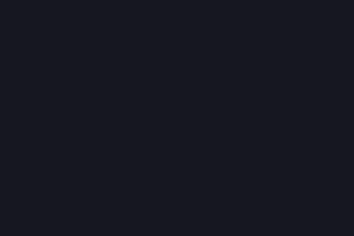
\includegraphics[width=55mm]{images/fig_sample.png}}
    \label{fig:pca_check_anechoic}
    \subfigure[PCA real data]{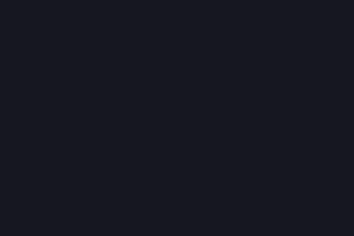
\includegraphics[width=55mm]{images/fig_sample.png}}
    \label{fig:pca_check_real}
    \caption{Result of PCA}
    \label{fig:pca_check}
\end{figure}

このように、両者は似たような変化をしていることがわかる。この変化にサポートベクターは着目しているため、無響室でのモデルが実環境のデータに当てはめることができたと考えられる。

次に、パラメトリック固有空間法をもちいて解析を行う。この手法を用いるために、第一主成分から第三主成分までの主成分を3軸として3次元プロットを行う。このような方法は、実際のデータに今回のような物理的な変化がある際に用いることで、3次元プロットした際にある規則的な動きをすることがあり、そこからモデル化の道筋を立てることができる。
今回の場合、角度が-50から50で回転しているため、回転のような連続的な動きが見れることが望ましい。
無響室データ、実環境データそれぞれの結果を\figref{pes_check}に示し、このときの、主成分分析の寄与率をTable. \ref{tab:pes_contri}に示す。

\begin{figure}[tb]
    \centering
    \subfigure[Parametric eigen space method of anechoic data]{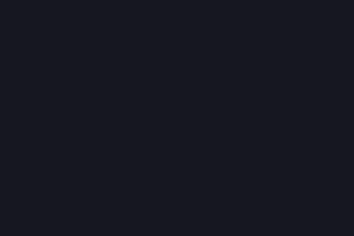
\includegraphics[width=55mm]{images/fig_sample.png}}
    \label{fig:pes_check_anechoic}
    \subfigure[Parametric eigen space method of real data]{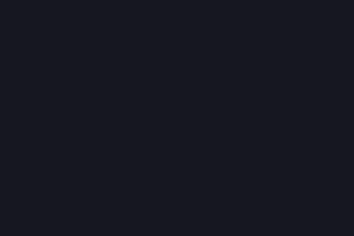
\includegraphics[width=55mm]{images/fig_sample.png}}
    \label{fig:pes_check_real}
    \caption{Parametric eigen space method}
    \label{fig:pes_check}
\end{figure}

\begin{table}[t]
    \centering
    \caption{Contribution rate}
    \vspace{1zh}
    \begin{tabular}{|c||p{4em}|p{4em}|} \hline
        PC & Anechoic & Real \\ \hline\hline
        PC1 & 0.73 & 0.52 \\ \hline
        PC2 & 0.18 & 0.13 \\ \hline
        PC3 & 0.03 & 0.05 \\ \hline
        SUM & 0.91 & 0.68 \\ \hline
    \end{tabular}
    \label{tab:pes_contri}
\end{table}

以上の結果より、確かに取得した音データの中には方位角による連続的な関係があることはわかった。さらに、動きもなめらかに円を描くような結果を出力している。このような点より、方位角と反射音の周波数領域の大きさには連続的な関係が見ることはできる。このため、サポートベクターによる回帰が可能であったと考えられる。

しかし、この図よりモデルを作成するのに必要な情報を取得することはできず、モデルベースで解くことは現状難しい。今回は可聴域の音波を最初の理由より用いていたが、今後は超音波を使用することを考えたい。理由としては、超音波は直進性が強いため可聴域よりも光の特性に似ている。こういった理由より、モデルベースで解く場合には超音波を用いることが良いと考えている。

\clearpage
\newpage
